\subsection{Trusted Execution Environment} \label{section:counter-external-tee}
%START TEXT INPUT
This is my real text! Rest might be copied or not be checked!
%START TEXT INPUT

WAS IST ES?
WAS MACHT ES?
WIE IMPLEMENTIERT MAN?
\url{https://source.android.com/security/trusty/index.html}
%
promoted as be all end all solution for mobile security
in theory isolated processing core with isolated memory, cannot be influenced by the outside and runs with priviliged acces
allows secure processing in the "secure world" that the "Normal world" cannot influence or beware of
senisitve processing offloaded to protect information from malware

perfect wish:
secure chip to process software that malware should not access, security related stuff like bankin, encryption

example Trustzone, Knox
\begin{figure}[h]
    \centering
    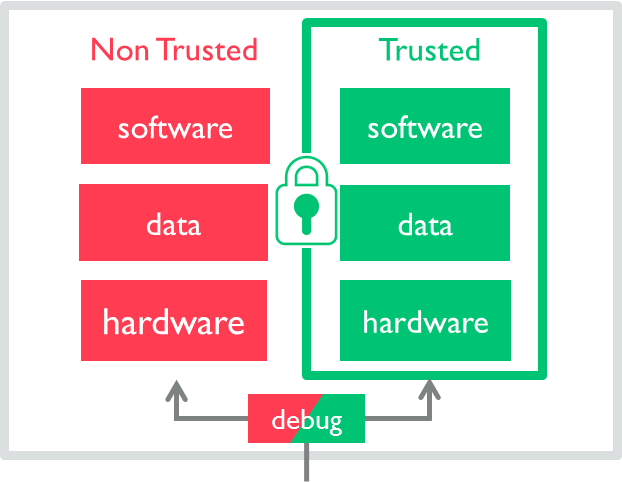
\includegraphics[width=0.8\textwidth]{data/tee.png}
    \caption{tee \cite{armTz}}
    \label{fig:tee}
\end{figure}


\cite{dragonTZ}\cite{armTz}
%



beispiele:
new section trusted execution environment
trusttronic letzte conference
samsung knox


%eval
luckypatcher not able to attack because it cannot access the TEE but before using it as a safe solution soem problems have to be fixed

%
e.g. trustzone
what is it already used for
secure data storage, hardware configurations, bootloader/sim lock
no hide from malware but user

architecture problems
kernel to your kernel
trustzone image stored unencrypted
pyhsical memory pointers

protection
validation can be done by either using qualcomms or writing a custom

one giant box, error by one has impact on all others

\cite{dragonTZ}\cite{armTz}
%

not accessible to anybody
in general many different solutions, focus should be on one unique standard in order to fix the problems and make compatibility , google already started by integrating features of samsung's knox into android lollipop \cite{samsungKnox}
